\chapter{Implementacja}
\section{Framework}
W ramach pracy powstała minibiblioteka zawierająca moduły ułatwiające implementację protokołów działających w ramach WSN. Stanowi ona rozszerzenie biblioteki INET, zawierającej moduły dla standardu IEEE 802.15.4.

Biblioteka składa się z następujących modułów:
\begin{itemize}
	\item WSNNode --- złożony moduł ,,abstrakcyjny'' stanowiący bazę dla węzłów sieci. W jego skład wchodzą:
\paragraph{Moduł mobilności} Jest to moduł zarządzający położeniem oraz mobilnością węzła. Jako, że zakres pracy obejmuje węzły stacjonarne, jako wartość domyślna został przyjęty moduł StationaryMobility, który jedynie śledzi położenie węzła.
\paragraph{Źródło energii} Jako źródło energii wykorzystany został udostępniony przez Inet moduł prostego zasobnika energii (SimpleEnergyStorage).
\paragraph{Tablica interfejsów} Przechowuje informacje o interfejsach danego węzła. W przypadku objątych tą pracą symulacji jest to jeden interfejs radiowy.
\paragraph{Moduł stanu węzła} Jest to moduł informujący o aktualnym stanie węzła.
\paragraph{Moduł monitora} Jest to autorski moduł monitorujący poziom energii w węźle do celów statystycznych. Moduł w regularnych odstępach czasu emituje sygnał zawierający aktualną ilość energii w węźle.
\paragraph{Moduł warstwy sieciowej} Odpowiada za warstwę sieciową węzła. Zawierają się w nim moduły odpowiedzialne za trasowanie pakietów.
\paragraph{Moduł karty sieciowej} Jest to moduł symulujący kartę sieciową. Zawiera się w nim moduł odpowiadający za warstwę fizyczną oraz moduł łącza danych.
\begin{figure}[!htbp]
	\begin{center}
		\centering
		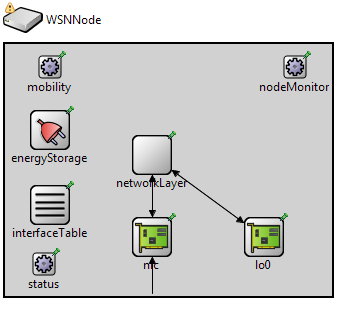
\includegraphics[scale=1]{\ImgPath/framework/node.png} 
	\end{center}
	\caption{Węzeł sieci}
	\label{abstractNode}
\end{figure}
\FloatBarrier
	\item WSNSensorNode - dziedziczy po WSNNode oraz zawiera dodatkowo moduł generujący pakiety
	\begin{figure}[!htbp]
	\begin{center}
		\centering
		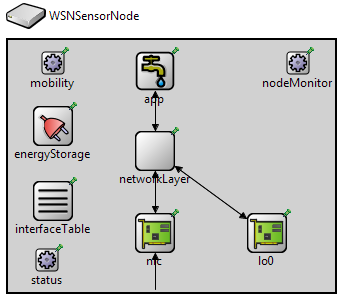
\includegraphics[scale=1]{\ImgPath/framework/sensor.png} 
	\end{center}
	\caption{Czujnik}
	\label{openlayers}
\end{figure}
\FloatBarrier
	\item WSNSinkNode - dziedziczy po WSNNode oraz zawiera dodatkowo moduł akcetujący pakiety od czujników
	\begin{figure}[!htbp]
	\begin{center}
		\centering
		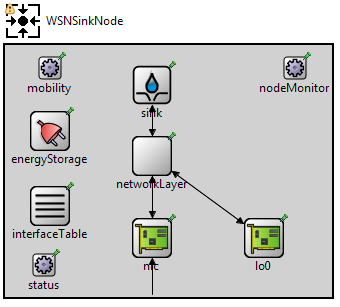
\includegraphics[scale=1]{\ImgPath/framework/sink.png} 
	\end{center}
	\caption{Stacja bazowa}
	\label{abstractNode}
\end{figure}
\FloatBarrier
	\item NodeCounter - moduł liczący działające węzły w sieci
	\item SimpleEnergyConsumer - moduł pobierający energię na żądanie
	\item VolatileStateBasedEnergyConsumer - moduł pobierający energię w zależności od ustawionego stanu z możliwością dynamicznej zmiany poboru mocy
\end{itemize}
\section{Protokoły}
Każda implementacja wybranego algorytmu trasowania wymaga stworzenia dwóch modułów. Jeden z nich dziedziczy po SimpleNetworkLayer, a drugi po NetworkProtocolBase.

Głównymi funkcjami, które jednocześnie wywoływane są przez silnik symulacji są handleSelfMessage, handleUpperPacket oraz handleLowerPacket.

\begin{minted}{cpp}
    virtual void handleSelfMessage(cMessage *msg) override;
    /** @brief Handle messages from upper layer */
    virtual void handleUpperPacket(cPacket *) override;

    /** @brief Handle messages from lower layer */
    virtual void handleLowerPacket(cPacket *) override;
\end{minted}
% flood jako akapit
\subsection{Flood}
W implementacji protokołu Flood wykorzystany został istniejący już moduł z biblioteki INET. Należało jedynie utworzyć  moduł będący warstwą sieciową, a następnie skonfigurować go, aby wykorzystywał moduł Flood z biblioteki INET.
\subsection{SPIN}
Protokół SPIN został zaimplementowany zgodnie z zaproponowanym w artykule \cite{Kulik2002} wariancie SPIN-RL.

Kod odpowiadający za logikę protokołu znajduje się w klasie SPIN, która dziedziczy po klasie NetworkProtocolBase oraz implementuje interfejs INetworkProtocol z biblioteki INET.

\begin{minted}{cpp}
class SPIN : public NetworkProtocolBase, public INetworkProtocol
\end{minted}

Moduł po otrzymaniu pakietu z wyższej warstwy dokonuje decyzji, czy węzeł ma dostatecznie dużo energii, aby przeprowadzić negocjację. W przypadku pozytywnej decyzji rozpoczynany jest proces negocjacji. W przeciwnym wypadku dane rozgłaszane są bezpośrednio, z pominięciem negocjacji.

\begin{minted}{cpp}
void SPIN::handleUpperPacket(cPacket *m)
{
    SPINDatagram *msg = encapsMsg(m, DATA);
    msg->setSeqNum(seqNum);
    seqNum++;

    if (isNegotiationViable()) {
        advertiseData(msg);
    } else {
        simpleSend(msg);
    }
    nbDataPacketsSent++;
}
\end{minted}

Algorytm decyzyjny przedstawiony jest na poniższym listingu.

\begin{minted}{cpp}
bool SPIN::isNegotiationViable()
{
    double randomNumber = uniform(0, 1);
    double currentEnergy = energyStorage->getResidualCapacity().get();
    double k = -1.2;
    double currentEnergyFrac = currentEnergy / maxEnergy;

    return randomNumber < (k*currentEnergyFrac / (k - currentEnergyFrac + 1));
}
\end{minted}

\begin{minted}{cpp}
std::map<MsgMetadata, SPINDatagram*, MsgMetadataCompare> 
    queuedMessages;
std::map<MsgMetadata, SPINDatagram*, MsgMetadataCompare> 
    queuedRequests;
std::set<MsgMetadata, MsgMetadataCompare> knownMessages;
std::set<MsgMetadata, MsgMetadataCompare> requestedMessages;
\end{minted}

\begin{minted}{cpp}
    void advertiseData(SPINDatagram *msg);
    void scheduleReq(MsgMetadata metadata, L3Address advertiser);
\end{minted}
\subsection{LEACH}
\begin{minted}{cpp}
void LEACH::handleUpperPacket(cPacket *m)
{
    if (!isSink) {
        LEACHPacket *netPacket = encapsMsg(m, LEACH_DATA_PACKET);
        if (!isCH && endFormClus) {
            CHInfo info = *CHcandidates.begin();
            netPacket->setDestAddr(info.src);
            bufferPacket(netPacket);
        } else if (!isCH && !endFormClus) {
            tempTXBuffer.push(netPacket);
        } else if (isCH) {
            bufferAggregate.push_back(netPacket);
        }
    }
}
\end{minted}

\begin{minted}{cpp}
case LEACH_DATA_PACKET:
            dest = msg->getDestAddr();
            if (isCH && interfaceTable->isLocalAddress(dest)) {
                bufferAggregate.push_back(msg);
            } else if (interfaceTable->isLocalAddress(dest) && isSink) {
                unpackAndSendUp(msg);
            } else {
                delete msg;
            }
break;
\end{minted}

\begin{minted}{cpp}
case LEACH_ADV_PACKET:
            if (!isCH && !isSink) {
                CHInfo rec;
                rec.src = msg->getSrcAddr();
                rec.rssi = rssi;
                CHcandidates.push_front(rec);
            }
            delete msg;
break;
\end{minted}

\begin{minted}{cpp}
case LEACH_JOIN_PACKET:
            dest = msg->getDestAddr();
            if (isCH && interfaceTable->isLocalAddress(dest)) {
                clusterMembers.push_back(msg->getSrcAddr());
            }
            delete msg;
break;
\end{minted}

\begin{minted}{cpp}
case LEACH_TDMA_PACKET:
            if (!isCH && !isSink) {
                clusterLength = msg->getScheduleArraySize();
                slotLength = roundLength*0.9 / clusterLength;
                for (int i = 0; i < clusterLength; i++) {
                    if (msg->getSchedule(i) == myNetwAddr) {
                        setStateSleep();
                        setTimer(START_SLOT, i * slotLength);
                        break;
                    }
                }
            }
            delete msg;
break;
\end{minted}
\subsection{ALEACH}
\begin{minted}{cpp}
void ALEACH::selectCH()
{
    if (roundNumber >= (numSensors / expectedCHNum)) {
        roundNumber = 0;
        isCt = false;
        isCH = false;
    }

    double randomNumber = uniform(0, 1);
    if (isCH) {
        isCH = false;
        isCt = true;
    }
    double generalProb = (double)expectedCHNum / (double)(numSensors - expectedCHNum * (roundNumber % (numSensors / expectedCHNum) ));
    double currentEnergy = energyStorage->getResidualCapacity().get();
    double currentStateProb = (currentEnergy / maxEnergy) * ((double) expectedCHNum / numSensors);
    if (isCt) {
        probability = 0;
    } else {
        probability = generalProb + currentStateProb;
    }
    if (randomNumber < probability) {
        isCH = true;
    }
}
\end{minted}
\subsection{LEACH DCHS}
\begin{minted}{cpp}
void LEACH_DCHS::selectCH()
{
    if (roundNumber >= (1 / percentage)) {
        roundNumber = 0;
        isCt = false;
        isCH = false;
    }

    double randomNumber = uniform(0, 1);
    if (isCH) {
        isCH = false;
        isCt = true;
    }
    double currentEnergy = energyStorage->getResidualCapacity().get();
    if (isCt) {
        probability = 0;
    } else {
        probability = percentage / (1 - percentage * (roundNumber % (int)(1/percentage)))
                * (currentEnergy / maxEnergy + (notCHRounds / (1/percentage)) * (1 - (currentEnergy / maxEnergy)));
    }
    if (randomNumber < probability) {
        isCH = true;
        notCHRounds = 0;
    } else if (!isCt) {
        ++notCHRounds;
    }
}
\end{minted}
\section{Poprawa biblioteki INET}
Umożliwienie warstwie sieciowej dostępu do rssi. Problem został już wcześniej zasygnalizowany przez jednego z użytkowników, jednakże nie został on rozwiązany. Znajomość rssi jest niezbędna do prawidłowego działania algorytmów opartych na LEACH.

Dodanie możliwości zmiany modułu MAC w Ieee802154NarrowbandNic.

Poprawa modułu IPvXTrafGen, tak aby prawidłowo zachowywał się podczas deaktywacji węzła.

Uzupełnienie modułu CSMA o funkcje obsługujące jego wyłączenie oraz ponowne włączenie. Przed poprawką, wyłącznie się symulowanego węzła (w wyniku zużycia energii) powodowało wystąpienie wyjątku i awaryjne zakończenie symulacji.

Obsługę przypadku, gdy pakiet dociera do wyłączonego już węzła.

Przeniesienie trzech poprawek autorstwa Floriana Kauera dotyczących szczegółów związanych z danymi zaczerpniętymi ze specyfikacji mikrokontrolera na podstawie której zdefiniowano domyślne parametry w Inecie.